
\documentclass[tikz]{standalone}

\definecolor{solarizedBlue}{HTML}{268BD2}
\definecolor{solarizedGreen}{HTML}{8DC73E}
\definecolor{solarizedViolet}{HTML}{6C71C4}
\definecolor{solarizedMagenta}{HTML}{D33682}

\usetikzlibrary{positioning, decorations.pathreplacing, backgrounds, fit, calc,matrix, arrows,scopes}


\begin{document}
\tikzset{man/.pic={
    \node[circle,fill,minimum size=10mm] (head) {};
    \node[rounded corners=4pt,minimum height=1.2cm,minimum width=0.8cm,fill,below = 2pt of head] (body) {};
    \draw[line width=2mm,round cap-round cap] ([shift={(4pt,-2pt)}]body.north east) --++(-90:6mm);
    \draw[line width=2mm,round cap-round cap] ([shift={(-4pt,-2pt)}]body.north west)--++(-90:6mm);
    }}
\begin{tikzpicture}

% \node (a) at (0, .1) {\textbf{a)}};

\node[align=center] (0) at (2, -1.5) {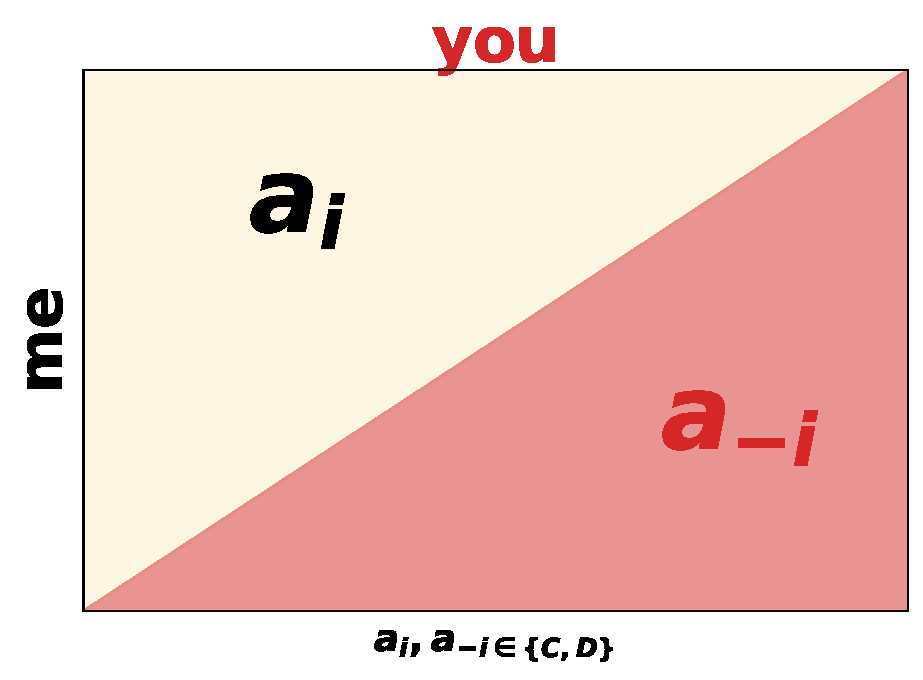
\includegraphics[width=.3\textwidth]{action_matrix.pdf}};

% panel b
% \node (b) at (5, .1) {\textbf{b)}};

% memory -  1
\pic[solarizedBlue] at (6, -1) (myman) {man};
\node[align=center] (0) at (8, -.5) {
\includegraphics[width=.2\textwidth]{memory_one.png}};
\node at (6, -3) (myman) {\textcolor{solarizedBlue}{memory$-1$}};


% panel c
% \node (c) at (0, -4) {\textbf{c)}};

% reactive -  1
\pic[solarizedGreen] at (1, -5) (myman) {man};
\node[align=center] (0) at (2.5, -4.5) {
\includegraphics[width=.2\textwidth]{reactive_n.png}};
\node at (1, -7) (myman) {\textcolor{solarizedGreen}{$n-$bit reactive}};


% panel d
% \node (d) at (5, -4) {\textbf{d)}};

% reactive -  1
\pic[solarizedViolet] at (6, -5) (myman) {man};
\node[align=center] (0) at (7.5, -4.5) {
\includegraphics[width=.2\textwidth]{self_reactive_n.png}};
\node at (6, -7) (myman) {\textcolor{solarizedViolet}{$n-$bit self reactive}};

\end{tikzpicture}
\end{document}